%% LyX 2.1.4 created this file.  For more info, see http://www.lyx.org/.
%% Do not edit unless you really know what you are doing.
\documentclass[english]{article}
\usepackage{charter}
\renewcommand{\familydefault}{\rmdefault}
\usepackage[T1]{fontenc}
\usepackage[utf8]{inputenc}
\usepackage{fancyhdr}
\pagestyle{fancy}
\usepackage{babel}
\usepackage{array}
\usepackage{graphicx}
\usepackage{setspace}
\onehalfspacing
\usepackage[unicode=true,pdfusetitle,
 bookmarks=true,bookmarksnumbered=false,bookmarksopen=false,
 breaklinks=false,pdfborder={0 0 0},backref=false,colorlinks=false]
 {hyperref}

\makeatletter

%%%%%%%%%%%%%%%%%%%%%%%%%%%%%% LyX specific LaTeX commands.
%% Because html converters don't know tabularnewline
\providecommand{\tabularnewline}{\\}

%%%%%%%%%%%%%%%%%%%%%%%%%%%%%% Textclass specific LaTeX commands.
\newenvironment{lyxlist}[1]
{\begin{list}{}
{\settowidth{\labelwidth}{#1}
 \setlength{\leftmargin}{\labelwidth}
 \addtolength{\leftmargin}{\labelsep}
 \renewcommand{\makelabel}[1]{##1\hfil}}}
{\end{list}}

%%%%%%%%%%%%%%%%%%%%%%%%%%%%%% User specified LaTeX commands.
\usepackage{babel}
\usepackage{babel}
\usepackage{babel}
\usepackage{babel}
\usepackage{babel}
\usepackage{babel}








\usepackage{listings}
\renewcommand{\lstlistingname}{Listing}





\usepackage{listings}
\renewcommand{\lstlistingname}{Listing}



\usepackage{listings}
\renewcommand{\lstlistingname}{Listing}

\makeatother

\begin{document}

\title{Glassfish 4.1.1 - Code inspection}

\maketitle
\begin{center}
\includegraphics[height=0.3\textheight]{polimiLogo} 
\par\end{center}

\begin{center}
Daniele Grattarola (Mat. 853101) 
\par\end{center}

\begin{center}
Ilyas Inajjar (Mat. 790009) 
\par\end{center}

\begin{center}
Andrea Lui (Mat. 850680) 
\par\end{center}


\title{\pagebreak{}}

\tableofcontents{}

\pagebreak{}


\section{Introduction}


\subsection{Purpose}

This is the code inspection document for a subset of methods in the
Glassfish 4.1.1 JEE web-server project. The purpose of this document
is to report all code-related issues and compliances of the methods,
in relation to some coding practices and standards that will be defined
later in the document.

This document is intended for software engineers and programmers involved
in the project, as it could possibly identify a necessity for a code
cleanup or restructuring.


\subsection{Scope}

The Glassfish 4.1.1 project is divided into different modules, each
composed of numerous classes and methods.

The analysis that will be carried out in this document will only involve
the following 5 methods of the StatefulSessionContainer class (located
at Glassfish 4.1.1/appserver/ejb/ejb-container/src/main/java/com/sun/ejb/containers/
of the public Subversion repository of the project): 
\begin{enumerate}
\item destroyExtendedEMsForContext( SessionContextImpl sc ) 
\item \_getContextForInstance( byte {[}{]} instanceKey ) 
\item \_getContext( EjbInvocation inv ) 
\item doVersionCheck( EjbInvocation inv, Object sessionKey, SessionContextImpl
sc ) 
\item handleConcurrentInvocation( boolean allowSerializedAccess, EjbInvocation
inv, SessionContextImpl sc, Object sessionKey ) 
\end{enumerate}

\subsection{Definitions, acronyms, and abbreviations}

Throughout this document, the following definitions will be applied
without further explanations: 
\begin{itemize}
\item \textbf{JEE}: Java Enterprise Edition 
\end{itemize}

\subsection{Code standards and best practice}

The analysis that will be performed in this document will be centered
on the following code standards and best practice, which will be checked
for each method. The conventions are given in the form of a checklist
and can be found attached to this document in the ``Assignment 3
- Code inspection.pdf'' file.

\pagebreak{}


\section{Checklist}
\begin{itemize}
\item \textbf{Naming Convention}

\begin{lyxlist}{00.00.0000}
\item [{\textbf{5)}\_getContextForInstance@1454,\_getContext@1605}]~
\item [{\textbf{6)}\_getContext@1676}]~
\item [{\textbf{7)}@185,@304,@323,@325}]~
\end{lyxlist}
\item \textbf{Indention: }Nothing found
\item \textbf{Braces: }Nothing found
\item \textbf{File Organization}

\begin{lyxlist}{00.00.0000}
\item [{\textbf{12)}\_getContextForInstance@1480,\_getContext@1673}]~
\item [{\textbf{13)}doVersionCheck@1772}]~
\item [{\textbf{14)}handleConcurrentInvocation@1786}]~
\end{lyxlist}
\item \textbf{Wrapping Lines}

\begin{lyxlist}{00.00.0000}
\item [{\textbf{17)}\_getContext@1645,1652,handleConcurrentInvocation@1806}]~
\end{lyxlist}
\item \textbf{Comments}

\begin{lyxlist}{00.00.0000}
\item [{\textbf{18)}\_getContext@1602}]~
\item [{\textbf{19)}\_getContextForInstance@1476,1477}]~
\end{lyxlist}
\item \textbf{Java Source Files: }Nothing found
\item \textbf{Package and Import Statements: }Nothing found
\item \textbf{Class and Interface Declarations}

\begin{lyxlist}{00.00.0000}
\item [{\textbf{25)}@278}]~
\item [{\textbf{27)}\_getContext@1605}]~
\end{lyxlist}
\item \textbf{Initialization and Declarations}

\begin{lyxlist}{00.00.0000}
\item [{\textbf{29)}doVersionCheck@1754,handleConcurrentInvocation@1786}]~
\end{lyxlist}
\item \textbf{Method Calls: }Nothing found
\item \textbf{Arrays: }Nothing found
\item \textbf{Object Comparison: }Nothing found
\item \textbf{Output Format}

\begin{lyxlist}{00.00.0000}
\item [{\textbf{43)}\_getContextForInstance@1471,}] doVersionCheck@1778
\end{lyxlist}
\item \textbf{Computation, Comparisons and Assignments: }Nothing found
\item \textbf{Exceptions}

\begin{lyxlist}{00.00.0000}
\item [{\textbf{52)}destroyExtendedEMsForContext@1395}]~
\end{lyxlist}
\item \textbf{Flow of Control}

\begin{lyxlist}{00.00.0000}
\item [{\textbf{54)}\_getContextForInstance@1476}]~
\item [{\textbf{56)}\_getContextForInstance@1462}]~
\end{lyxlist}
\item \textbf{Files: }Nothing found
\end{itemize}

\section{Methods}


\subsection{destroyExtendedEMsForContext\label{sub:destroyExtendedEMsForContext}}

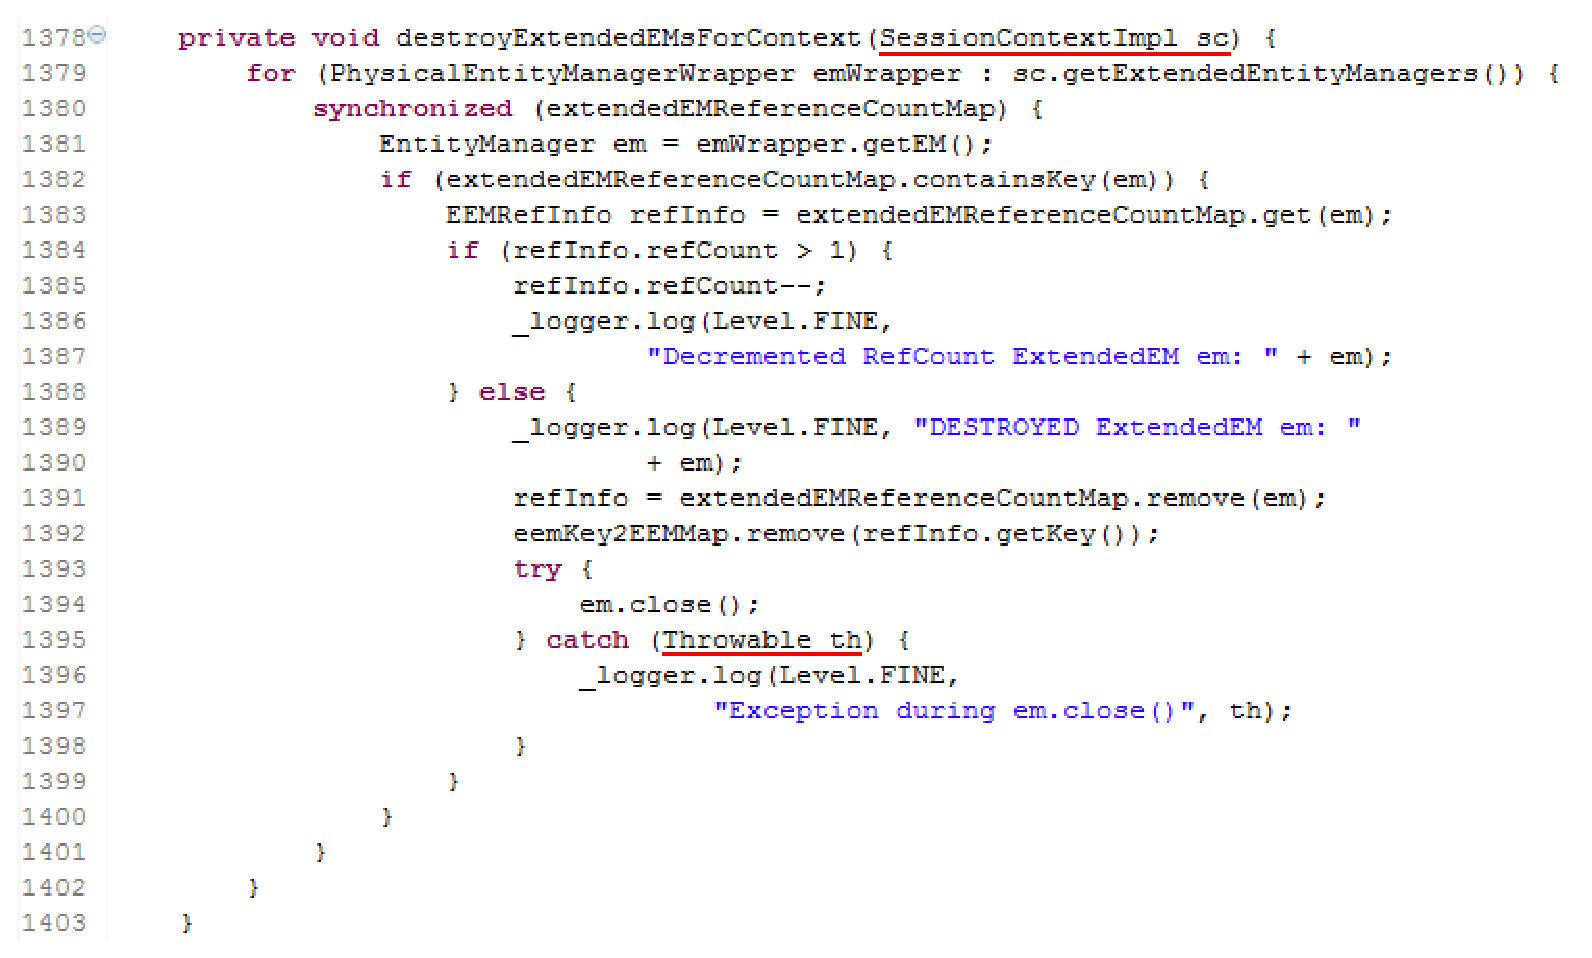
\includegraphics[width=1\textwidth]{destroyExtendedEMsForContext}


\subsection{\_getContextForInstance\label{sub:_getContextForInstance}}

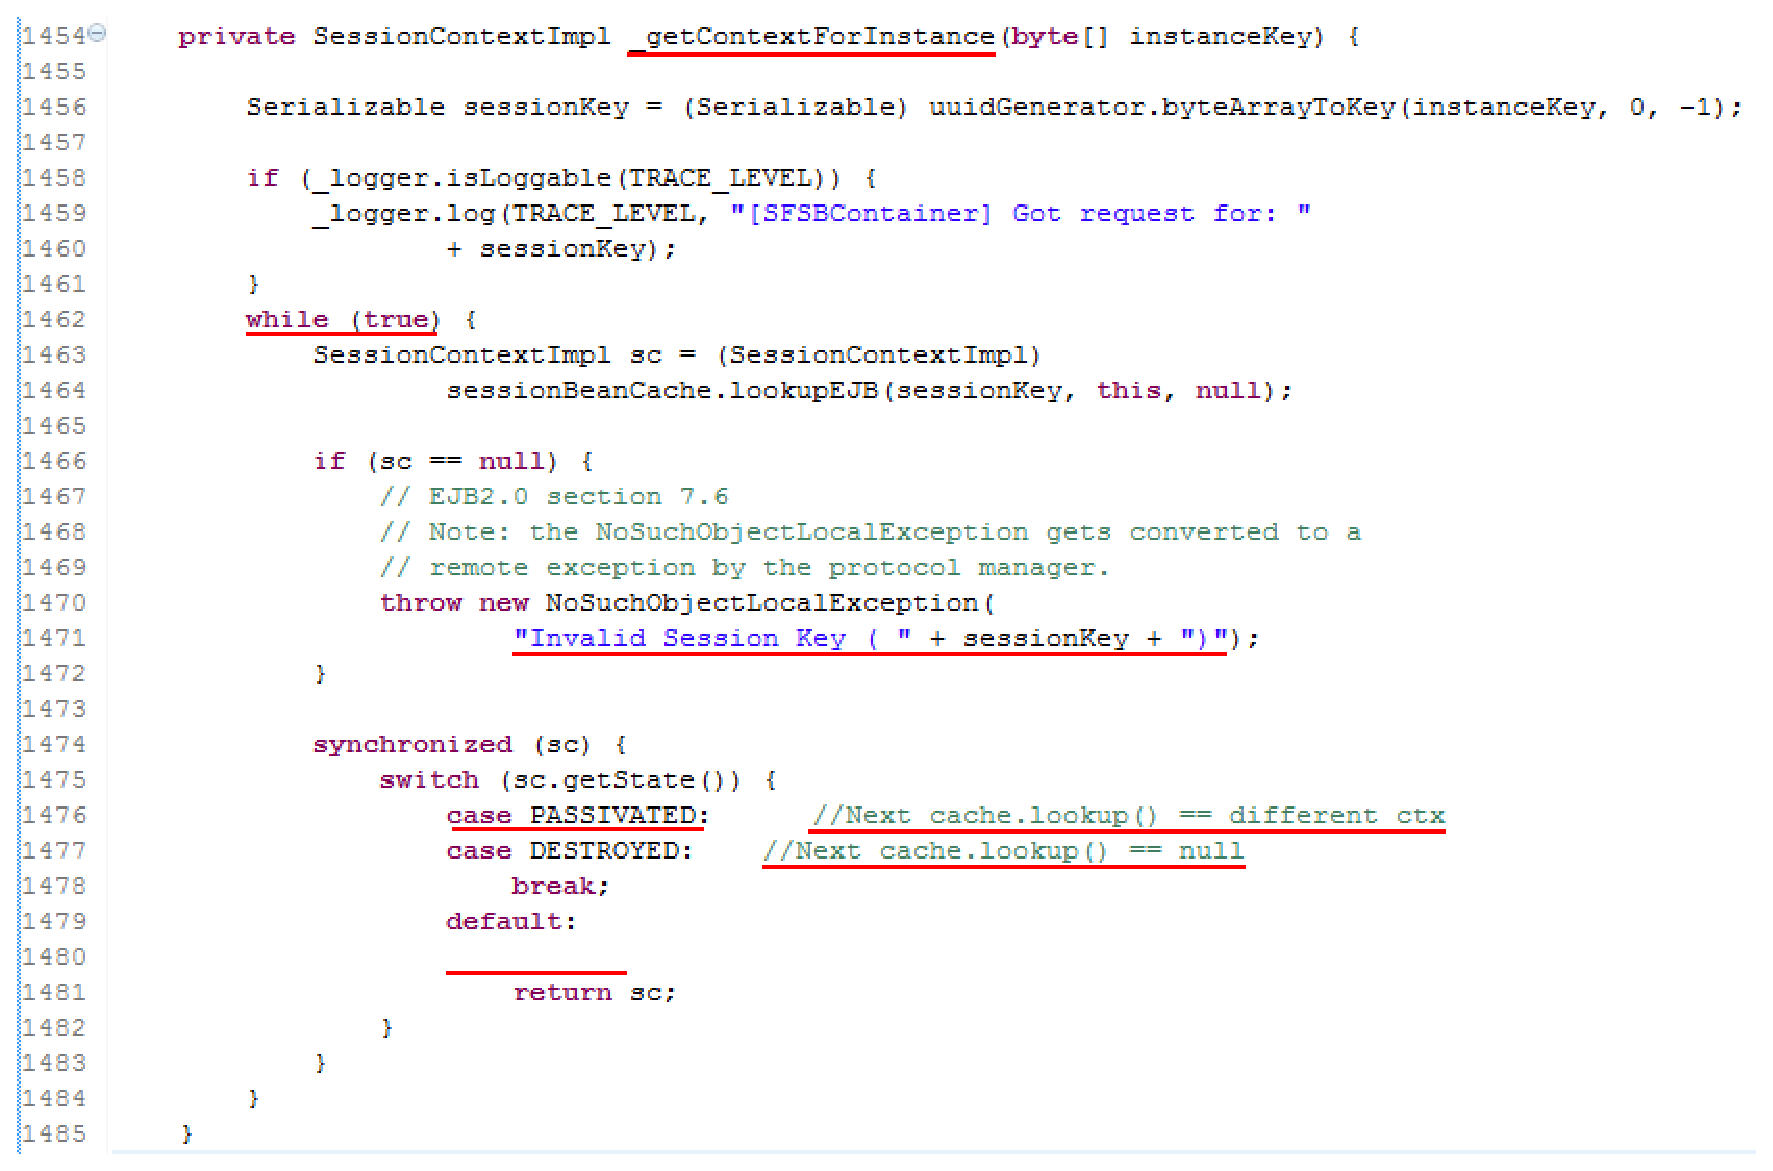
\includegraphics[width=1\textwidth]{_getContextForInstance}


\subsection{\_getContext\label{sub:_getContext}}

\includegraphics[width=1\textwidth]{_getContext1}

\includegraphics[width=1\textwidth]{_getContext2}

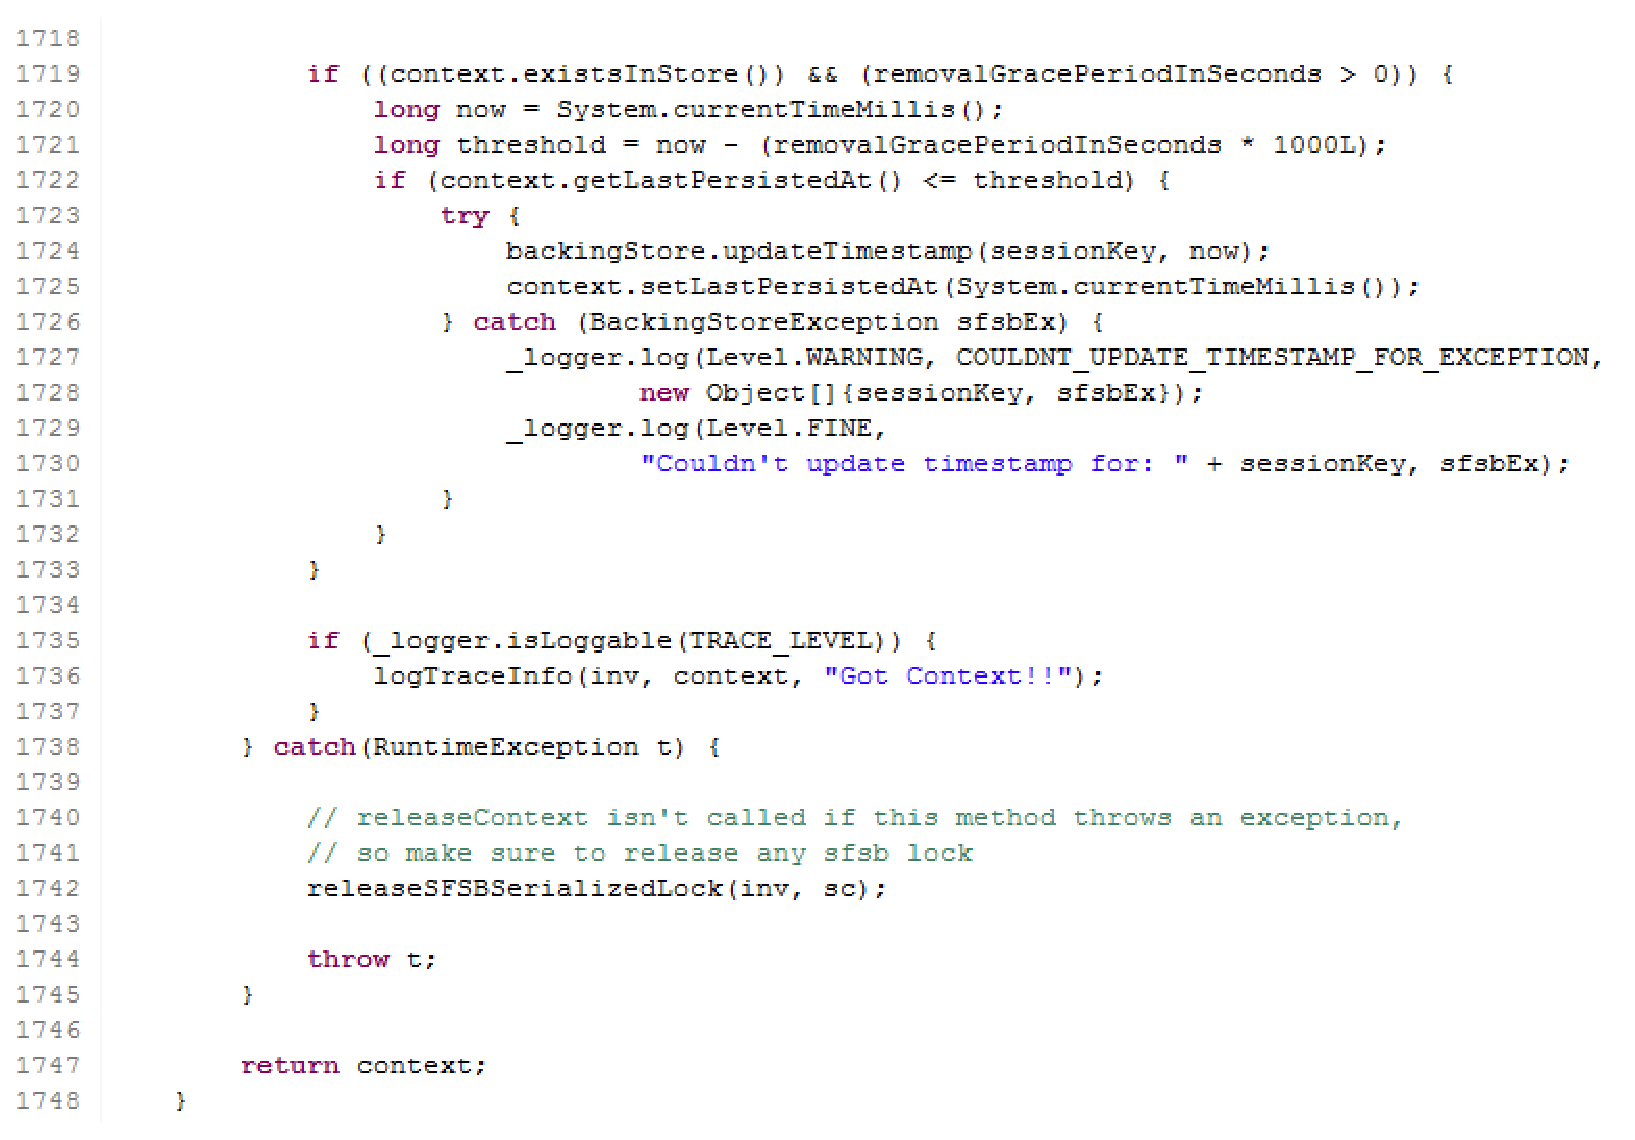
\includegraphics[width=1\textwidth]{_getContext3}


\subsection{doVersionCheck\label{sub:doVersionCheck}}

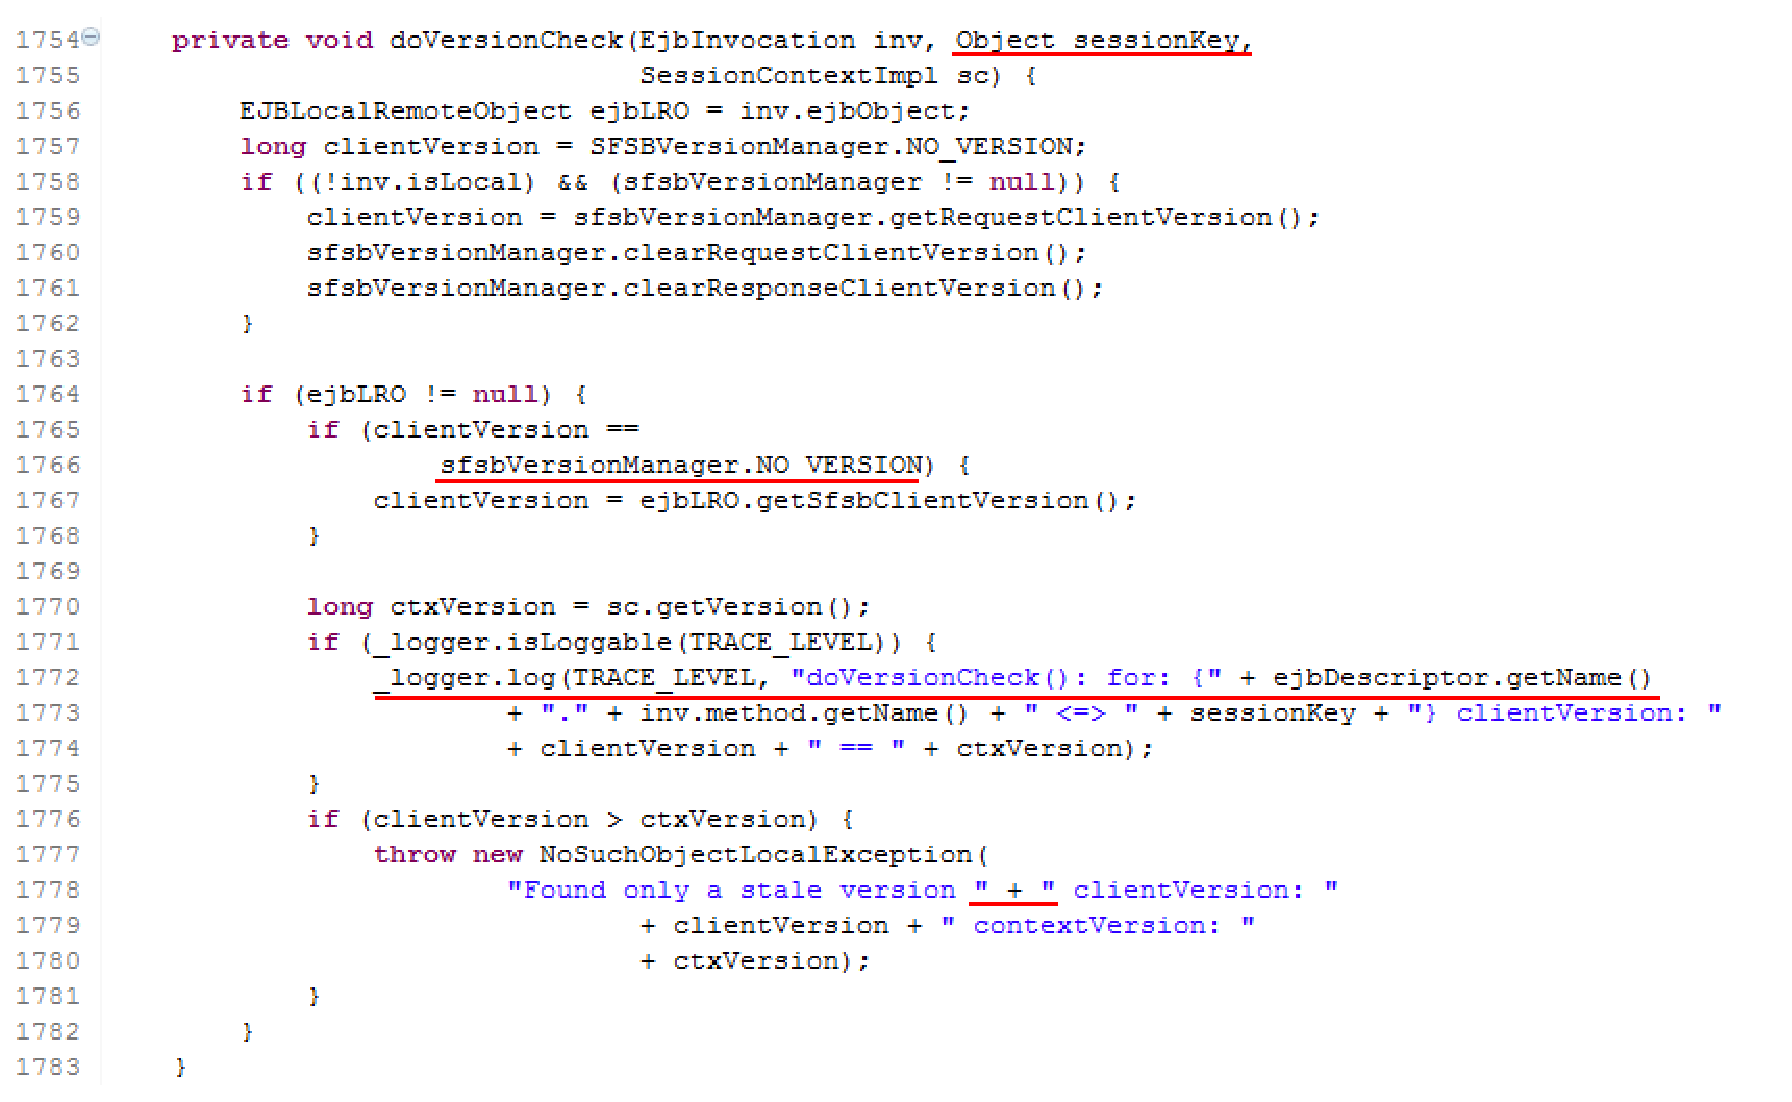
\includegraphics[width=1\textwidth]{doVersionCheck}


\subsection{handleConcurrentInvocation\label{sub:handleConcurrentInvocation}}

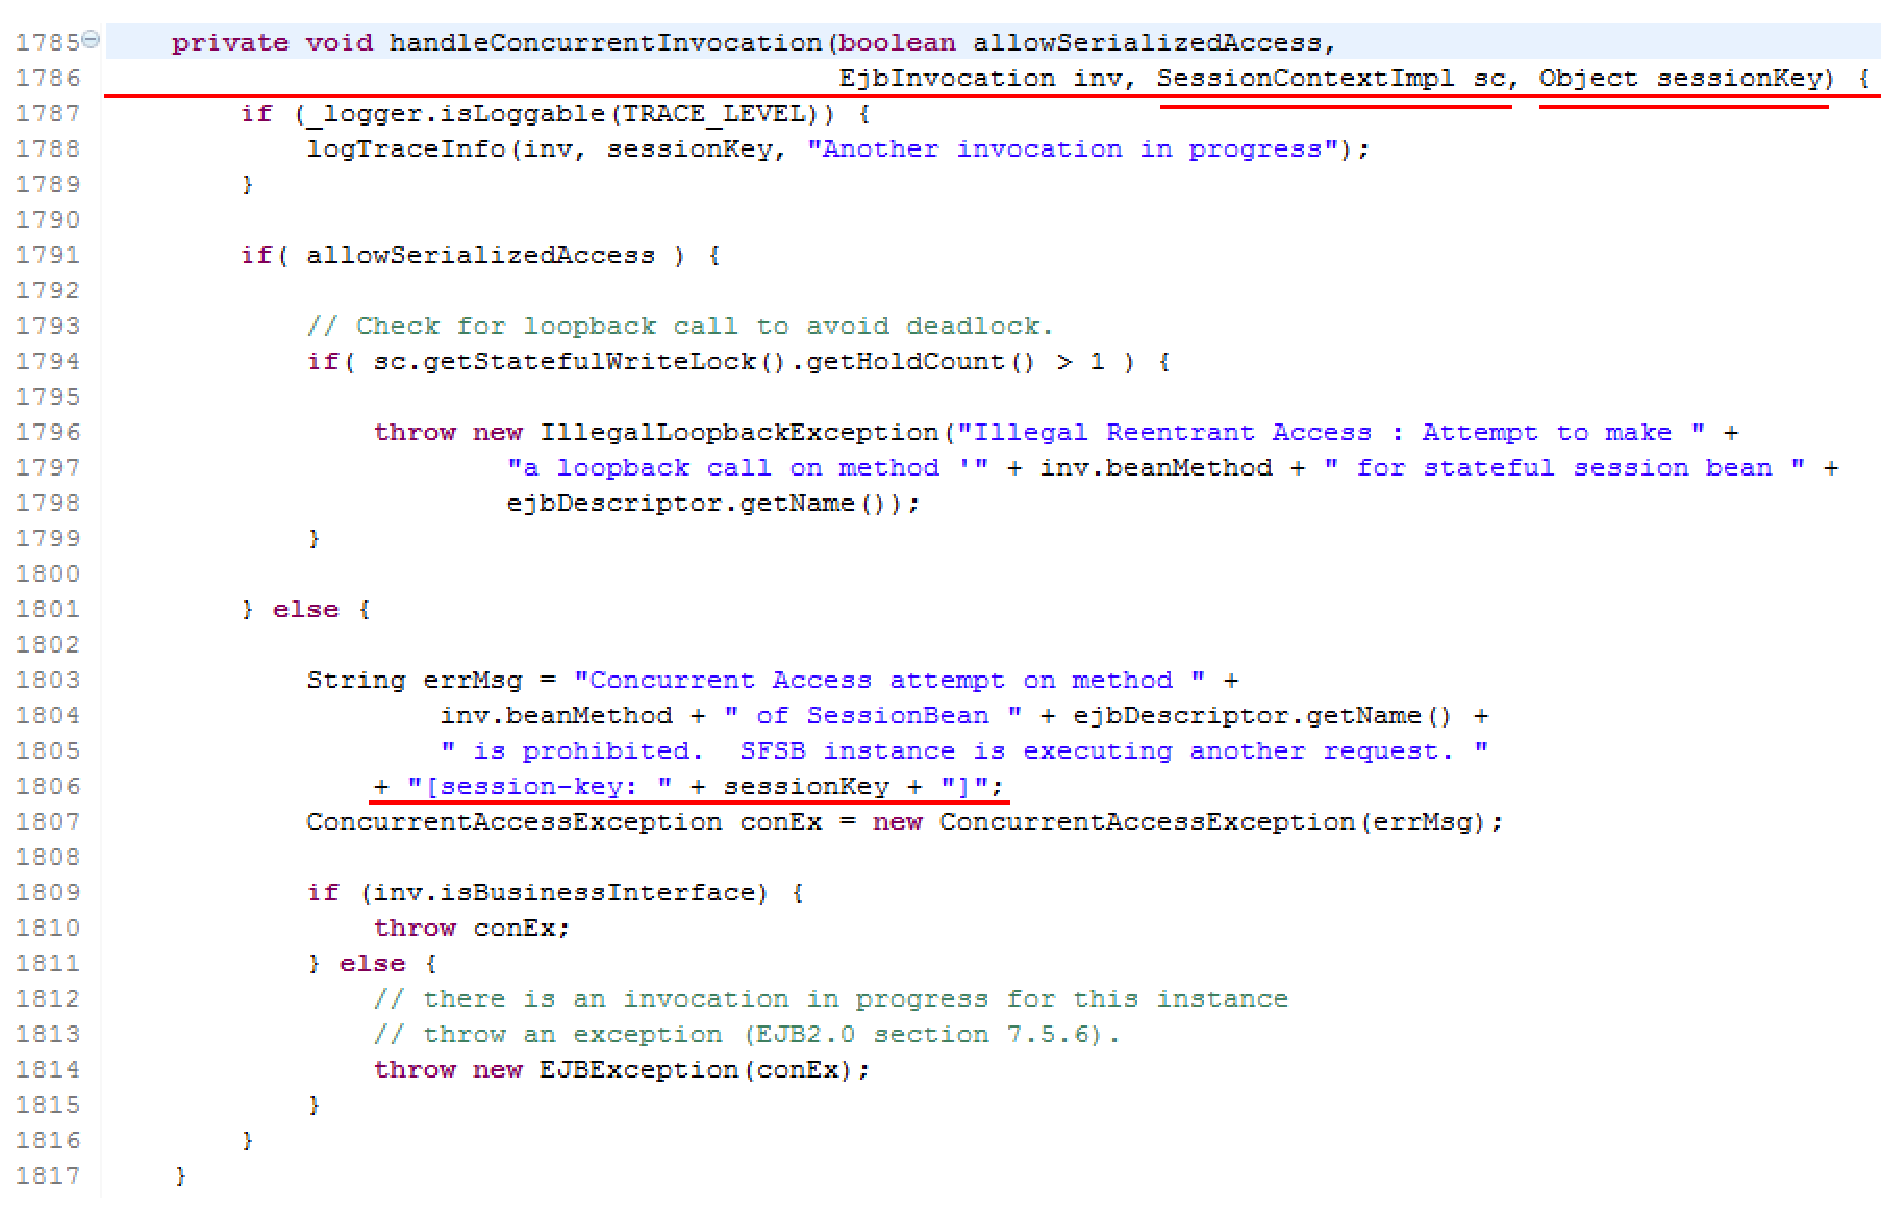
\includegraphics[width=1\textwidth]{handleConcurrentInvocation}


\section{Code inspection}


\subsection{StatefulSessionContainer}

\begin{tabular}{lc>{\raggedright}p{8cm}}
\hline 
\multicolumn{1}{|l|}{\textbf{Line}} & \multicolumn{1}{c|}{\textbf{Checklist Number}} & \multicolumn{1}{>{\raggedright}p{8cm}|}{\textbf{Comment}}\tabularnewline
\hline 
185 & 7 & Last character not uppercase \tabularnewline
\hline 
278 & 25 & public static variable after private static ones \tabularnewline
\hline 
304 & 7 & non costant variable with uppercase name \tabularnewline
\hline 
323 & 7 & constant with lowecase name \tabularnewline
\hline 
325 & 7 & constant with lowecase name \tabularnewline
\hline 
\end{tabular}


\subsection{destroyExtendedEMsForContext}

\begin{tabular}{lc>{\raggedright}p{8cm}}
\hline 
\multicolumn{1}{|l|}{\textbf{Line}} & \multicolumn{1}{c|}{\textbf{Checklist Number}} & \multicolumn{1}{>{\raggedright}p{8cm}|}{\textbf{Comment}}\tabularnewline
\hline 
1378 &  & Instead using parameter SessionContextImpl use List of PhysicalEntityManagerWrapper \tabularnewline
\hline 
1395 & 52 & Catch block catch Throwable instead of Illegal State Exception \tabularnewline
\hline 
\end{tabular}


\subsection{\_getContextForInstance}

\begin{tabular}{cc>{\raggedright}p{8cm}}
\hline 
\multicolumn{1}{|c|}{\textbf{Line}} & \multicolumn{1}{c|}{\textbf{Checklist Number}} & \multicolumn{1}{>{\raggedright}p{8cm}|}{\textbf{Comment}}\tabularnewline
\hline 
1454 & 5 & Method name pattern should be {[}a-z{]}{[}a-z0-9{]}{[}a-zA-Z0-9\_{]}{*} \tabularnewline
\hline 
1462 & 56 & While(true) loop \tabularnewline
\hline 
1471 & 43 & Incorrect output format \tabularnewline
\hline 
1476 & 54 & Empty case block without break or return \tabularnewline
\hline 
1476 & 19 & Commented line of code \tabularnewline
\hline 
1477 & 19 & Commented line of code \tabularnewline
\hline 
1480 & 12 & Useless blank line \tabularnewline
\hline 
\end{tabular}


\subsection{\_getContext}

\begin{tabular}{cc>{\raggedright}p{8cm}}
\hline 
\multicolumn{1}{|c|}{\textbf{Line}} & \multicolumn{1}{c|}{\textbf{Checklist Number}} & \multicolumn{1}{>{\raggedright}p{8cm}|}{\textbf{Comment}}\tabularnewline
\hline 
1602 & 18 & Comment not explain adequately the method functions \tabularnewline
\hline 
1605 & 27 & Duplication Code lines: 1621, 1677, 1696. Can be avoided with a proper
method \tabularnewline
\hline 
1605 & 5 & Method name pattern should be {[}a-z{]}{[}a-z0-9{]}{[}a-zA-Z0-9\_{]}{*} \tabularnewline
\hline 
1645 & 17 & Wrong indentation and duplicated '+' \tabularnewline
\hline 
1652 & 17 & Wrong indentation and duplicated '+' \tabularnewline
\hline 
1673 & 12 & Useless blank line \tabularnewline
\hline 
1676 & 6 & Abbreviation in name must contain no more than one capital letter \tabularnewline
\hline 
\end{tabular}


\subsection{doVersionCheck}

\begin{tabular}{cc>{\raggedright}p{8cm}}
\hline 
\multicolumn{1}{|c|}{\textbf{Line}} & \multicolumn{1}{c|}{\textbf{Checklist Number}} & \multicolumn{1}{>{\raggedright}p{8cm}|}{\textbf{Comment}}\tabularnewline
\hline 
1754 & 29 & Useless paramether (sessionKey) used only for log \tabularnewline
\hline 
1766 &  & Static refence to a non static object \tabularnewline
\hline 
1772 & 13 & Line can be less then 80 characters \tabularnewline
\hline 
1778 & 43 & String concatenation can be avoided \tabularnewline
\hline 
\end{tabular}


\subsection{handleConcurrentInvocation}

\begin{tabular}{cc>{\raggedright}p{8cm}}
\hline 
\multicolumn{1}{|c|}{\textbf{Line}} & \multicolumn{1}{c|}{\textbf{Checklist Number}} & \multicolumn{1}{>{\raggedright}p{8cm}|}{\textbf{Comment}}\tabularnewline
\hline 
1786 & 14 & Lines can be less then 80 characters \tabularnewline
\hline 
1786 & 29 & Useless parameters: SessionContextImpl, 'sessionKey' only for log \tabularnewline
\hline 
1806 & 17 & Splitted line not aligned\tabularnewline
\hline 
\end{tabular}

\pagebreak{}


\section{Additional comments}

The production of this document has been a joint effort of all the
authors, with a fair distribution of the mansions which caused each
member of the group to work on all the parts of the document. The
production has been carried out between 9/12/2015 and 4/1/2016 for
a total time expense of: 
\begin{itemize}
\item \textbf{Group work}: 6 hours 
\item \textbf{Individual work}:


\begin{tabular}{|c|c|}
\hline 
Daniele Grattarola (Mat. 853101)  & 3hours\tabularnewline
\hline 
Ilyas Inajjar (Mat. 790009)  & 3hours\tabularnewline
\hline 
Andrea Lui (Mat. 850680)  & 5hours\tabularnewline
\hline 
\end{tabular}\end{itemize}

\end{document}
